\section{Ход работы}
1. Измерены температура в помещении и внешнее давление. Так как погрешности приборов даны не были, будем считать, что их не было.
\[T = 27.8 ^\circ C,\]
\[p_\text{атм} = 100.17 \text{ кПа}.\]

2. Измерены объем запертого между кранами К$_5$ и К$_6$ воздуха, давление откачано до $p_1$, измерено давление после открытия крана К$_6$.
\[V_\text{К$_5$ и К$_6$} = 50 \text{ см}^3,\]
\[p_1 = 1.4 \cdot 10^{-2} \text{ торр},\]
\[p = \rho g\Delta h = 885 \frac{\text{кг}}{\text{м}^3} \cdot 9.81 \frac{\text{м}}{c^2} \cdot \left(257 \pm 1\right) \text { мм} = \left(2231 \pm 8\right) \text{ Па}.\]

3. Пользуясь законом Бойля-Мариотта можно найти объем форвакуумной части:
\[p_\text{атм} V_\text{К$_5$ и К$_6$} = p \cdot \left(V_\text{К$_5$ и К$_6$} + V_\text{фв}\right),\]
\[V_\text{фв} = V_\text{К$_5$ и К$_6$}\cdot\left(\frac {p_\text{атм}} p - 1\right) = \left(2195 \pm 8\right) \text{ см}^3.\]

4. Аналогично рассчитан объем всей установки и высоковакуумной части:
\[V_\text{вся установка} = \left(3475 \pm 22\right) \text{ см}^3,\]
\[V_\text{вв} = \left(1230 \pm 23\right) \text{ см}^3.\]

5. Измерено предельное давление в системе $p_\text{пр} = 0.62 \cdot 10^{-4} \text{ торр}$.

6. Измерена зависимость давления при ухудшении и улучшении ваккума, данные представлены в табл. 1.
По этой зависимости построен график с уравнением $p - p_\text{пр} = 0,0474t + 0,1176$.

7. Построена зависимость для случая улучшения в табл.2.
По этой зависимости построен график с уравнением $\ln(p - p_\text{пр}) = -0,1786t + 1,9051$.

8. Получим скорость откачки диффузионного насоса (q -- наклон графика):
\[W = -q\cdot V = (22 \pm 2) \cdot 10^{-2} \text{ л}/c.\]

9. Получим значение $Q_\text{н}$, уравнение принимает вид:
\[V_\text{вв}dP = \left(Q_\text{д} + Q_\text{н}\right) dt.\]
Так в этом случае $Q_\text{д}$ имеет порядок $10^{-8}$, $Q_\text{д} + Q_\text{н} \approx Q_\text{н}$. Таким образом,
\[Q_\text{н} = \frac{dp}{dt} V_\text{вв} = (58 \pm 5) \text{ торр}\cdot \text{л} / c\]

10. Рассчитаем $W$ другим способом:
\[P_\text{пр}W = Q_1, \text{    } P_\text{уст}W = Q_1 + \frac{d\left(PV\right)}{dt}.\]
Из (6):
\[W = \frac{\frac{4}{3}(d/2)^3\sqrt{\frac{2\pi RT}{\mu}}\frac{P_\text{фв}}{L}}{p_\text{уст} - p_\text{пр}} = 21 \cdot 10^{-2} \text{ л}/c.\]



\begin{table}[h]
\centering
\begin{tabular}[h]{|c|c|c|c|c|c|c|c|}
        \hline
        t, c & p,  $10^{-4}$ торр & t, c & p,  $10^{-4}$ торр & t, c & p,  $10^{-4}$ торр & t, c & p,  $10^{-4}$ торр \\
        \hline
                0 & 0,05 & 1 & 0,05 & 2 & 0,09 & 3 & 0,12\\
        \hline
        4 & 0,17 & 5 & 0,17 & 6 & 0,29 & 7 & 0,35\\
        \hline
        8 & 0,38 & 9 & 0,38 & 10 & 0,48 & 11 & 0,58\\
        \hline
        12 & 0,68 & 13 & 0,68 & 14 & 0,78 & 15 & 0,78\\
        \hline
        16 & 0,88 & 17 & 0,88 & 18 & 0,98 & 19 & 0,98\\
        \hline
        20 & 1,08 & 21 & 1,08 & 22 & 1,18 & 23 & 1,18\\
        \hline
        24 & 1,28 & 25 & 1,28 & 26 & 1,38 & 27 & 1,38\\
        \hline
        28 & 1,48 & 29 & 1,48 & 30 & 1,58 & 31 & 1,58\\
        \hline
        32 & 1,68 & 33 & 1,68 & 34 & 1,78 & 35 & 1,78\\
        \hline
        36 & 1,88 & 37 & 1,88 & 38 & 1,98 & 39 & 1,98\\
        \hline
        40 & 2,08 & 41 & 2,08 & 42 & 2,18 & 43 & 2,18\\
        \hline
        44 & 2,28 & 45 & 2,28 & 46 & 2,38 & 47 & 2,38\\
        \hline
        48 & 2,38 & 49 & 2,38 & 50 & 2,48 & 51 & 2,58\\
        \hline
        52 & 2,58 & 53 & 2,58 & 54 & 2,68 & 55 & 2,78\\
        \hline
        56 & 2,78 & 57 & 2,78 & 58 & 2,88 & 59 & 2,98\\
        \hline
        60 & 2,98 & 61 & 2,98 & 62 & 3,08 & 63 & 3,18\\
        \hline
        64 & 3,18 & 65 & 3,18 & 66 & 3,28 & 67 & 3,38\\
        \hline
        68 & 3,38 & 69 & 3,38 & 70 & 3,48 & 71 & 3,58\\
        \hline
        72 & 3,58 & 73 & 3,58 & 74 & 3,68 & 75 & 3,78\\
        \hline
        76 & 3,78 & 77 & 3,78 & 78 & 3,88 & 79 & 3,88\\
        \hline
        80 & 3,98 & 81 & 3,98 & 82 & 4,08 & 83 & 4,08\\
        \hline
        84 & 4,18 & 85 & 4,18 & 86 & 4,28 & 87 & 4,28\\
        \hline
        88 & 4,28 & 89 & 4,28 & 90 & 4,38 & 91 & 4,48\\
        \hline
        92 & 4,48 & 93 & 4,48 & 94 & 4,58 & 95 & 4,68\\
        \hline
        96 & 4,68 & 97 & 4,68 & 98 & 4,78 & 99 & 4,78\\
        \hline
        100 & 4,88 & 101 & 4,88 & 102 & 4,98 & 103 & 4,98\\
        \hline
        104 & 5,08 & 105 & 5,08 & 106 & 5,18 & 107 & 5,18\\
        \hline
        108 & 5,18 & 109 & 5,18 & 110 & 5,28 & 111 & 5,38\\
        \hline
        112 & 5,38 & 113 & 5,38 & 114 & 5,48 & 115 & 5,58\\
        \hline
        116 & 5,58 & 117 & 5,58 & 118 & 5,68 & 119 & 5,68\\
        \hline
        120 & 5,78 & 121 & 5,78 & 122 & 5,88 & 123 & 5,88\\
        \hline
        124 & 5,98 & 125 & 5,98 & 126 & 5,98 & 127 & 6,08\\
        \hline
        128 & 6,08 & 129 & 6,08 & 130 & 6,18 & 131 & 6,28\\
        \hline
        132 & 6,28 & 133 & 6,28 & 134 & 6,38 & 135 & 6,38\\
        \hline
\end{tabular}
\caption{Зависимость давления от времени при ухудшении вакуума}
\end{table}
\begin{table}[h]
\centering
\begin{tabular}[h]{|c|c|c|c|c|c|}
    \hline
    t, c & $\ln (p - p_\text{пр})$ \\
    \hline
    0 & 1,83736998048011 \\
    \hline
    1 & 1,8213182714696 \\
    \hline
    2 & 1,73695123273306 \\
    \hline
    3 & 1,58514521986506 \\
    \hline
    4 & 1,38128181929635 \\
    \hline
    5 & 1,12492959698548 \\
    \hline
    6 & 0,867100487683383 \\
    \hline
    7 & 0,631271776841858 \\
    \hline
    8 & 0,392042087776024 \\
    \hline
    9 & 0,165514438477573 \\
    \hline
    10 & -0,0202027073175195 \\
    \hline
    11 & -0,2484613592985 \\
    \hline
    12 & -0,385662480811985 \\
    \hline
    13 & -0,544727175441672 \\
    \hline
    14 & -0,7339691750802 \\
    \hline
    15 & -0,967584026261706 \\
    \hline
    16 & -1,10866262452161 \\
    \hline
    17 & -1,27296567581289 \\
    \hline
    18 & -1,38629436111989 \\
    \hline
    19 & -1,51412773262978 \\
    \hline
    20 & -1,6094379124341 \\
    \hline
    21 & -1,71479842809193 \\
    \hline
    22 & -1,77195684193188 \\
    \hline
    23 & -1,83258146374831 \\
    \hline
\end{tabular}
\caption{Зависимость давления от времени при ухудшении вакуума}
\end{table}

\begin{figure}[h]
\centering
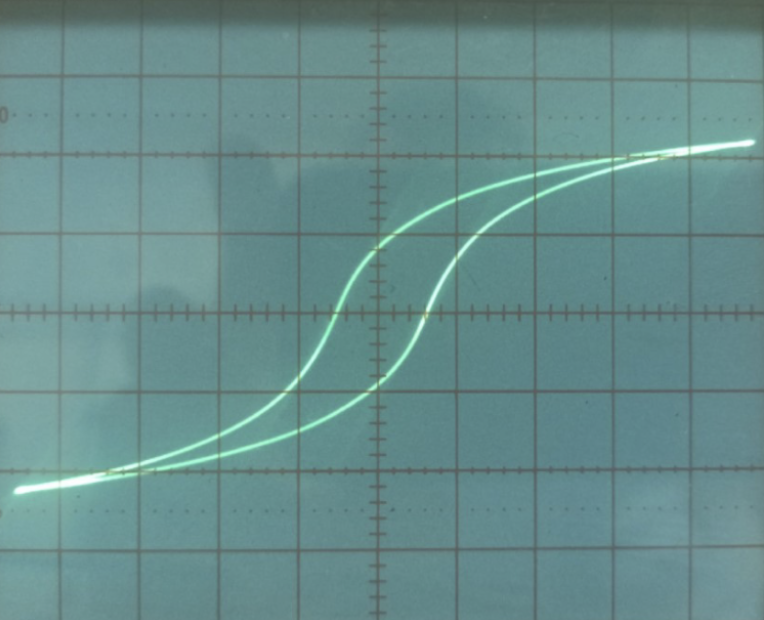
\includegraphics[width = \linewidth]{p3.png}
\caption{Ухудшение вакуума}
\end{figure}

\begin{figure}[h]
\centering
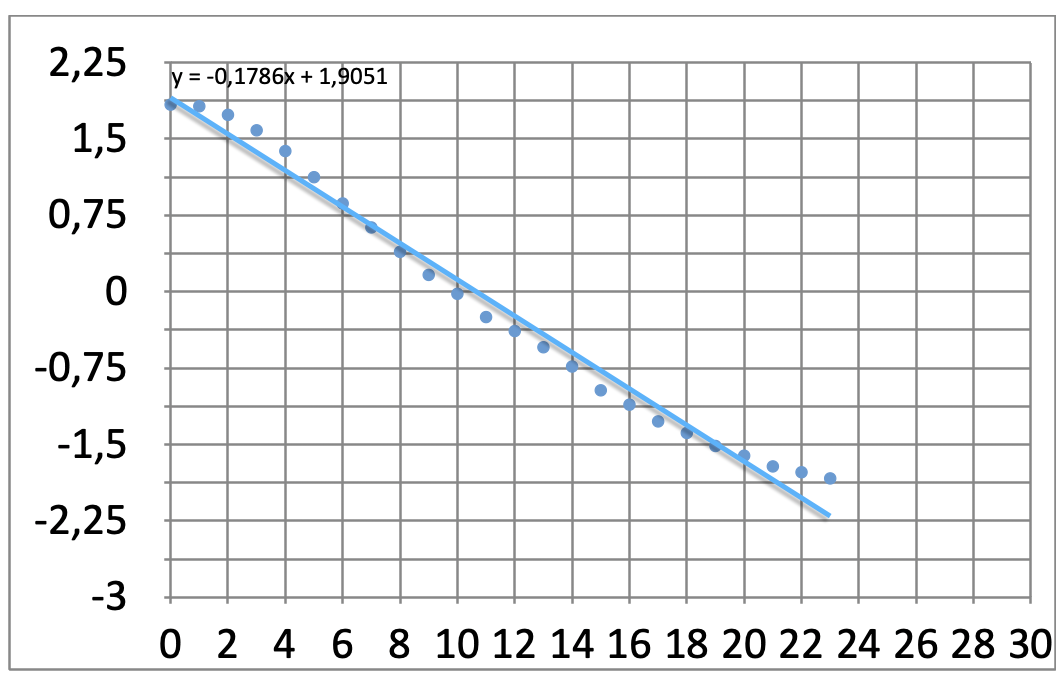
\includegraphics[width = \linewidth]{p4.png}
\caption{Улучшение вакуума}
\end{figure}
